\FILE{hadoop.tex}

\subsubsection{Map Reduce}

Map reduce models have been familiar to the programming and distrubted
computing community for a long time and have been historically often
associated with the functional programming's map and reduce. However
the map and reduce framework introduced recently \cite{Dean:mapreduce}
distinguishes itself from such efforts while
applying it repeatedly, with fault tollerance on a very large
distributed data set. 

Instead of bringing the data to the computer in map reduce application
we often use the concept of brinnging the computing to the data. This
makes a lot of sense when we assume that google has a large number of
data that is distributed an many serveres and repeated search queries
are cast to find results accross them. 

In general we can define a {\em map} step, that takes the input problem and divides it
into smaller sub-problems distributing it among worker nodes. The map
function is than executed on the data distributed on the various
servers. The {\em reduce} step collects the answers of the subproblem and combines
them in some fashion. 

\begin{figure}[htb]
  \centering
    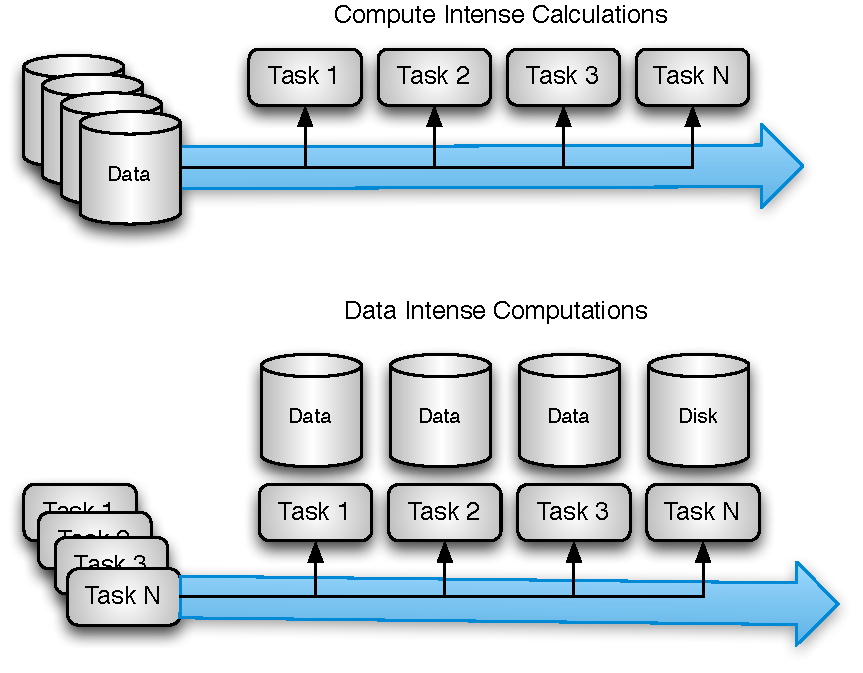
\includegraphics[width=1.0\textwidth]{images/mapreduce.pdf}
  \caption{Project Member Dist.}
\end{figure}

\paragraph{Hadoop}\label{S:hadoop}

Hadoop \cite{report/myhadoop}\cite{myhadoop2} is an Apache project
delivering an opensource software that uses the map/reduce farmework
in a distributed environment while focussing on scalability and
reliability. Its design includes the Hadoop FIle System providing an
easy to use file system to distribute the data among the servers on
which the caluculations will be executed. Hadoop is designed to deal
with faults through redundancy which is an important feature when
conducting data analysis on very large distributed databases
\cite{www/hadoop}.  Hadoop is written in Java and provides the
essential map reduce functionality and allows the system to be
configured for existing hardware.

\paragraph{myHadoop}

MyHadoop which is installed on many of the compute clusters in
FutureGrid, enables to launch Hadoop clusters via traditional
high-performance compute clusters. For this it utilizes the underlying
batch scheduling system. 

The reason for managing hadoop jobs via a batch system may be
multiple. First, the available infrastructure is resource constrained
and utilization of disks and compute resources must be specially
accounted for to allow shared usage by many users. This naturally
happens in the educational research community quite frequently. 
Second, to efficiently utilize the compute and data infrastructure
researchers may not run Hadoop or MPI jobs continiously. At times the
may need an haddop environment at other time they prefer a traditional
message passing enviironment while at the same time being under
resource constratints.

The idea of myHadoop is to submit a job to the queuing system that
sets up a hadoop cluster for the length of the reseravation and the
researcher can than use it do conduct experiments either via
predifined jobs or in interactive mode. This is achieved by
identifying a number of resources 



by first requesting resources
for an Nnode Hadoop cluster via PBS. Once the resources are received, the Hadoop
configurations and environments are set up based on the set of resources provided by
PBS. The Hadoop Distributed File System (HDFS) can be configured in one of two ways
– in 1) transient (nonpersistent) or 2) persistent modes. In the nonpersistent mode, the
HDFS is set up to use local storage. In the persistent mode, the HDFS is set to
symbolically link to an external location that will be persistent – i.e. data from Hadoop
runs will continue to persist even after the Hadoop runs are complete. More details are as
follows.

\paragraph{Details}

The prerequisite for myHadoop is a valid Hadoop installation – we recommend that you
use Hadoop version 0.20.2 since that is the only version of Hadoop that this package has
been tested with. Henceforth, we will refer to the location of the Hadoop installation as
HADOOP\_HOME. We will refer to the location of the myHadoop installation (i.e. this
package) as MY\_HADOOP\_HOME. The \$MY\_HADOOP\_HOME/pbs-example.sh shows
an example of how to use myHadoop with PBS. A similar script for SGE can be found in
\$MY\_HADOOP\_HOME/sge-example.sh.
A step-by-step process for using myHadoop is as follows.

\paragraph{Initial Configuration}

Ensure that the environment variables inside \$MY\_HADOOP\_HOME/bin/setenv.sh are
set correctly. You can set your HADOOP\_HOME, and the locations for your HDFS data
and log directories using this script. You will need to update this script before you can
proceed further.
All the tuning parameters for Hadoop can be found in the \$MY\_HADOOP\_HOME/etc
directory. There is no need to edit any of the parameters, especially if you are not an
expert Hadoop user. If you are familiar with the various Hadoop parameters, you may
edit the parameters that fall outside the “DO NOT EDIT” sections.

\paragraph{Request N nodes from the Scheduler}

Once the environment variables have been set correctly, we are ready to use myHadoop
using a regular PBS or SGE submission script. Your PBS script should contain the
following lines to initialize PBS as follows:

\begin{verbatim}
#!/bin/bash
#PBS -q <queue_name>
#PBS -N <job_name>
#PBS -l nodes=4:ppn=1
#PBS -o <output file>
#PBS -e <error_file>
#PBS -A <allocation>
#PBS -V
#PBS -M <user email>
#PBS -m abe
\end{verbatim}

In the above case, we are requesting 4 nodes. Note that you must set the processors per
node (ppn) to 1.
Your SGE script should contain the following lines to initialize SGE:

\begin{verbatim}
#!/bin/bash
#$ -V -cwd
#$ -N <job_name>
#$ -pe <queue_name> 4
#$ -o <output file>
#$ -e <error file>
#$ -S /bin/bash
\end{verbatim}

For SGE, there is one important rule to remember. The queue name specified above
should be preconfigured with an allocation\_rule set to 1 (one). This ensures that the
Hadoop cluster is set up such that multiple instances of the Hadoop daemons are not
scheduled on the same node.

\paragraph{Set the myHadoop Environment}

Run the \$MY\_HADOOP\_HOME/bin/setenv.sh script (that you modified in Section 2.1)
to set all the environment variables required by myHadoop.
. \$MY\_HADOOP\_HOME/bin/setenv.sh
Set the HADOOP\_CONF\_DIR to the directory where Hadoop configs should be
generated – all configuration files for the Hadoop run will be picked up from here. Ensure
that this directory is accessible to all nodes – and a way to do this is to make sure that this
directory is on a shared file system such as NFS or Lustre.
export HADOOP\_CONF\_DIR=<configuration directory>

\paragraph{Configure the myHadoop Cluster}

You can initialize and configure the Hadoop cluster by using the
\$MY\_HADOOP\_HOME/bin/pbs-configure.sh (or sge-configure.sh) script. You may
create a transient or persistent myHadoop cluster by changing the commandline
arguments as follows.
For a transient myHadoop cluster, configure it as follows (replace 4 with the total number
of nodes requested):
\$MY\_HADOOP\_HOME/bin/pbs-configure.sh -n 4 -c \$HADOOP\_CONF\_DIR
In this mode, you will have to copy all of your data into the myHadoop cluster after it is
configured, and copy out the results after the job is complete. All data will be
inaccessible from HDFS once the PBS job is complete.
Alternatively, you may set up a persistent myHadoop cluster by using the –p option, and
setting the BASE\_DIR for HDFS as follows:
\$MY\_HADOOP\_HOME/bin/pbs-configure.sh -n 4 -c \$HADOOP\_CONF\_DIR -p -d
<HDFS BASE\_DIR>
The BASE\_DIR should be on a directory accessible to all nodes, to ensure that the data
will not be cleaned up after job completion. For instance, the BASE\_DIR could be on a
Lustre file system. Note that, if N-node cluster is being created, then the BASE\_DIR
should have directories named 1, 2, … , N. The configuration script sets up symbolic
links from node I to the BASE\_DIR/I directory. When this mode is used, there is no need
to copy data back and forth from HDFS to another file system between runs.

\paragraph{Format HDFS (if need be)}

If myHadoop is being used in transient mode, or if it is being used for the first time in
persistent mode, then you will have to format the HDFS as follows:
\$HADOOP\_HOME/bin/hadoop --config \$HADOOP\_CONF\_DIR namenode –format

\paragraph{Run Hadoop Jobs}

You are now all set to start all the Hadoop daemons as follows:
\$HADOOP\_HOME/bin/start-all.sh
Once the daemons are all started up, you can start using Hadoop as usual. You may also
stage data in and out from HDFS, as required.

\paragraph{Clean up}

Although, PBS or SGE may be set up to automatically clean up after your Hadoop job is
complete, it is always a good idea to stop all the Hadoop daemons, and use the cleanup
script to clean up after yourself.
\$HADOOP\_HOME/bin/stop-all.sh
\$MY\_HADOOP\_HOME/bin/pbs-cleanup.sh -n 4 OR
\$MY\_HADOOP\_HOME/bin/sge-cleanup.sh -n 4


\paragraph{myHadoop}

MyHadoop is a set of scripts that configure and instantiate Hadoop as a batch job.

myHadoop 0.20.2 is currently installed on Alamo, Hotel, India, and Sierra FutureGrid systems.



We have various platforms that support Hadoop on FutureGrid. MyHadoop is probably the easiest solution offered for you. It provides the advantage that it is integrated into the queuing system and allows hadoop jobs to be run as batch job. This is of especial interest for classes that may run quickly out of resources if every students wants to run their hadoop application at the same time.



MapReduce is a programming model developed by Google. Their definition of MapReduce is as follows: “MapReduce is a programming model and an associated implementation for processing and generating large data sets. Users specify a map function that processes a key/value pair to generate a set of intermediate key/value pairs, and a reduce function that merges all intermediate values associated with the same intermediate key.” For more information about MapReduce, please see the Google paper here.

The Apache Hadoop Project provides an open source implementation of MapReduce and HDFS (Hadoop Distributed File System).

This tutorial illustrates how to run Apache Hadoop thru the batch systems on FutureGrid using the MyHadoop tool.


